% Latex template: mahmoud.s.fahmy@students.kasralainy.edu.eg
% For more details: https://www.sharelatex.com/learn/Beamer

\documentclass[aspectratio=1610]{beamer}					% Document class

\setbeamertemplate{footline}[text line]{%
  \parbox{\linewidth}{\vspace*{-8pt}Dynamics on gene networks \hfill\insertshortauthor\hfill\insertpagenumber}}
\setbeamertemplate{navigation symbols}{}

\usepackage[english]{babel}				% Set language
\usepackage[utf8x]{inputenc}			% Set encoding

\mode<presentation>						% Set options
{
  \usetheme{default}					% Set theme
  \usecolortheme{default} 				% Set colors
  \usefonttheme{default}  				% Set font theme
  \setbeamertemplate{caption}[numbered]	% Set caption to be numbered
}

% Uncomment this to have the outline at the beginning of each section highlighted.
%\AtBeginSection[]
%{
%  \begin{frame}{Outline}
%    \tableofcontents[currentsection]
%  \end{frame}
%}

\usepackage{graphicx}					% For including figures
\usepackage{booktabs}					% For table rules
\usepackage{hyperref}	
\usepackage{tikz-network}				% For cross-referencing
\usepackage[absolute,overlay]{textpos}
\usepackage{bm}
\usepackage[font=small,labelfont=bf]{caption}

\title{Isolating the perturbation response of gene regulatory networks in the presence of biological variability and technical noise}	% Presentation title
\author{Clayton W. Seitz}								% Presentation author
\date{\today}									% Today's date	

\begin{document}

% Title page
% This page includes the informations defined earlier including title, author/s, affiliation/s and the date
\begin{frame}
  \titlepage
\end{frame}

\begin{frame}{Outline}
  \tableofcontents
\end{frame}


% The following is the most frequently used slide types in beamer
% The slide structure is as follows:
%
%\begin{frame}{<slide-title>}
%	<content>
%\end{frame}

\begin{frame}{Gene expression is stochasic and non-constitutive}


\begin{textblock*}{7cm}(0.5cm,1.5cm)
\begin{figure}
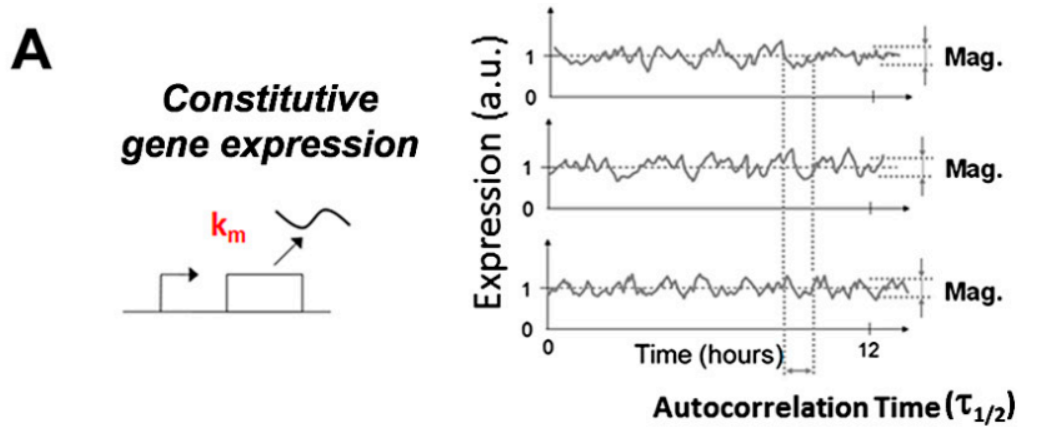
\includegraphics[width=7cm]{burst-1.png}
\end{figure}
\end{textblock*}

\begin{textblock*}{7cm}(8cm,1.5cm)
\begin{figure}
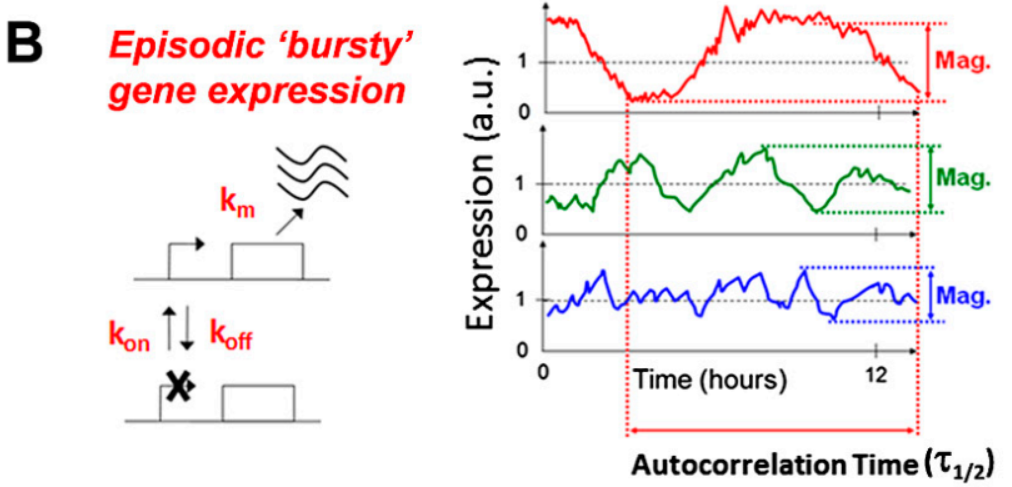
\includegraphics[width=7cm]{burst-2.png}
\end{figure}
\end{textblock*}


\begin{textblock*}{15cm}(0.5cm,6cm)
\begin{itemize}
\item If the biochemical network is known a-priori, we can build parametric dynamical models
\item Bayesian inference allows us to fit parametric dynamical models without continuous dynamical trajectories
\end{itemize}
\end{textblock*}


\end{frame}

\begin{section}{Modeling stochastic biochemical reaction networks}

\begin{frame}{Stochastic biochemical reaction networks: the repressilator}
\begin{textblock*}{10.5cm}(3cm,1cm)
\begin{figure}
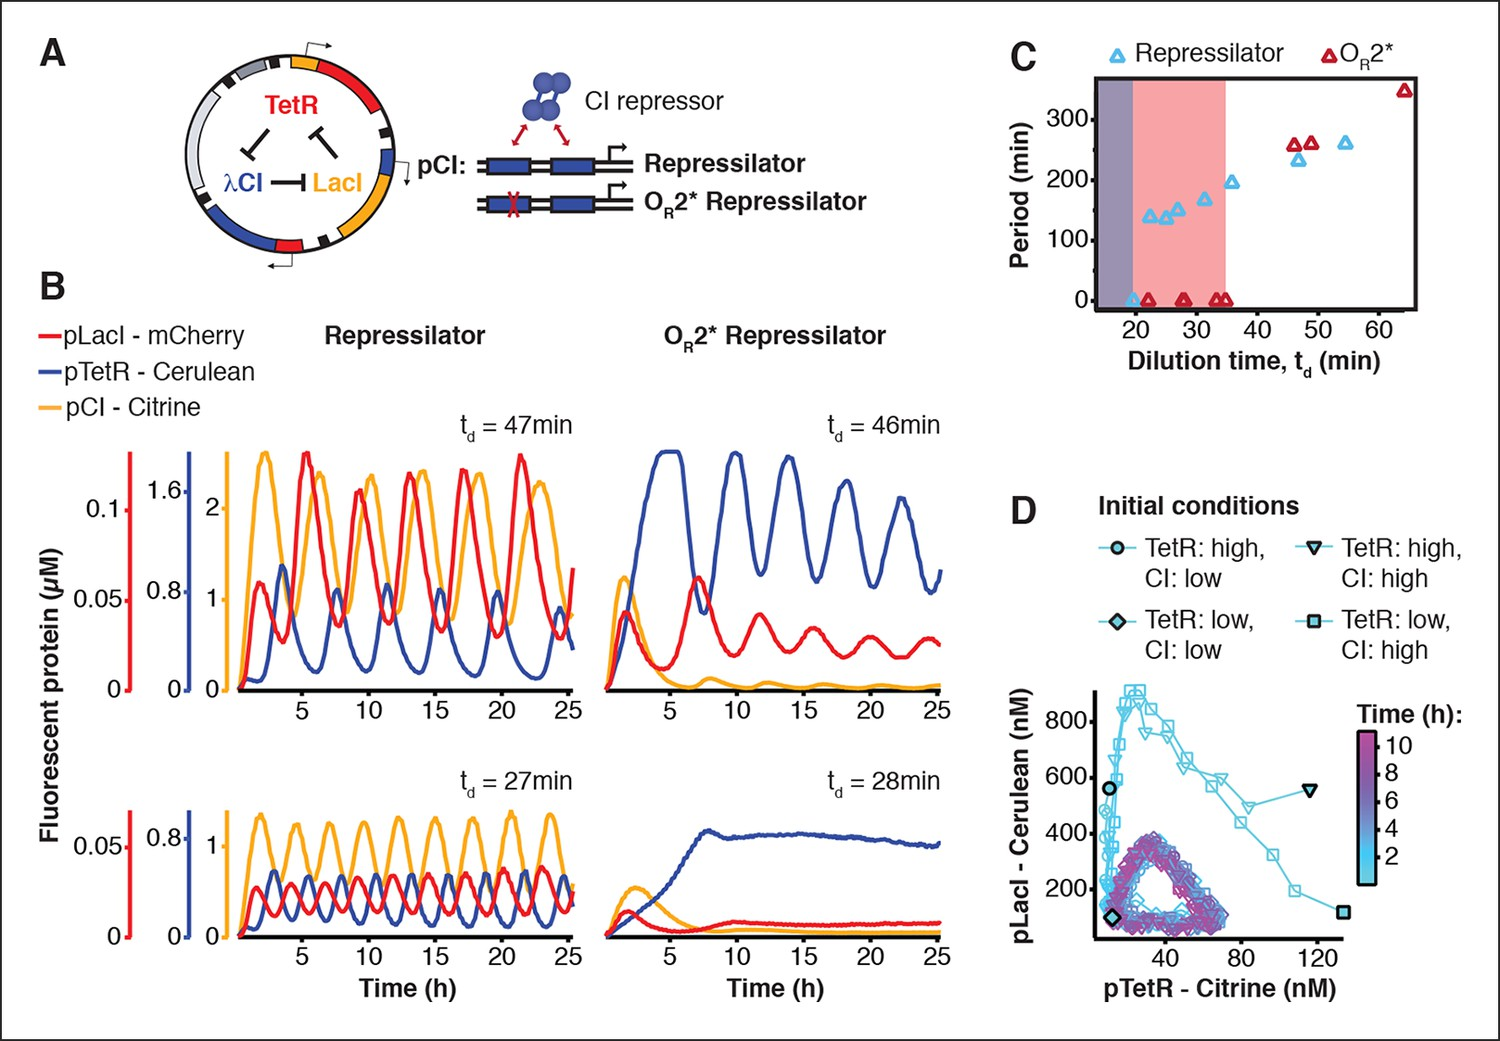
\includegraphics[width=10.5cm]{repressilator.jpg}
\caption{Niederholtmyer et al., eLife 2015}
\end{figure}
\end{textblock*}
\end{frame}


\begin{frame}{Kolmogorov's forward equation (chemical master equation)}

Dynamics on biochemical reaction networks are inherently stochastic and the state space is discrete. We can only write probabilities over the state space

\vspace{0.1in}

\begin{align*}
P(\mathbf{x}_{i},t) &= \sum_{j} T_{ji}(\mathbf{x}_{i},t|\mathbf{x}_{j},t-\Delta t)P(\mathbf{x}_{j},t-\Delta t)\\ 
&= \sum_{k} T_{k}(\mathbf{x}_{i},t|\mathbf{x}_{i}-\nu_{k},t-\Delta t)P(\mathbf{x}_{i}-\nu_{k},t-\Delta t)
\end{align*}

where $T_{k}$ is the probability of a reaction channel $k$ firing in the interval $(t,t+\Delta t)$.\\
\vspace{0.1in}
Taking the limit $\Delta t \rightarrow 0$ one can derive the forward Kolmogorov equation or chemical master equation (CME)

\begin{align*}
\frac{dP(\mathbf{x},t|\mathbf{x}_{0})}{dt} = \sum_{k} T_{k}(\mathbf{x}-\nu_{k})P(\mathbf{x}-\nu_{k},t) - T_{k}(\mathbf{x})P(\mathbf{x},t)
\end{align*}

\end{frame}

\begin{frame}{What about Markov models?}
From another point of view, since the dynamics are Markov the state $\mathbf{x}$ follows the DAG
\vspace{0.2in}

\begin{center}
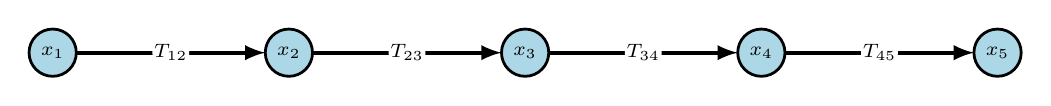
\begin{tikzpicture}
\Vertex[x=0,y=0,label=$x_{1}$]{A}
\Vertex[x=3,y=0,label=$x_{2}$]{B}
\Vertex[x=6,y=0,label=$x_{3}$]{C}
\Vertex[x=9,y=0,label=$x_{4}$]{D}
\Vertex[x=12,y=0,label=$x_{5}$]{E}
\Edge[Math,Direct=true,color=black,label=T_{12}](A)(B)
\Edge[Math,Direct=true,color=black,label=T_{23}](B)(C)
\Edge[Math,Direct=true,color=black,label=T_{34}](C)(D)
\Edge[Math,Direct=true,color=black,label=T_{45}](D)(E)
\end{tikzpicture}
\end{center}

For MMs, the EM algorithm can be used for MAP estimation, but this requires time-series measurements\\
\vspace{0.1in}
Time-series measurements in live cells severely limits the number of species considered simultaneously\\
\vspace{0.1in}
More often than not the data we have are \emph{ensemble snapshots}

\end{frame}

\begin{frame}{Bayesian parameter inference using ensemble snapshots}

Suppose we have a series of ensemble snapshots of an \emph{in-vitro} population:

\begin{align*}
\mathbf{x} = \{\mathbf{x}_{0}, ..., \mathbf{x}_{t}\}\;\;\; \mathbf{y} = \{\mathbf{y}_{0}, ..., \mathbf{y}_{t}\}
\end{align*}

with $\mathbf{x}_{t} = \{x_{1}, ..., x_{n}\}$ and similarly for $\mathbf{y}$. Under perfect measurements $\mathbf{x}=\mathbf{y}$\\
\vspace{0.2in}
We would like to use $\mathbf{x}$ to fit a dynamical model $\mathcal{M}(\theta)$. Bayesian inference lets us infer $\theta$ from $\mathbf{x}$ while quantifying the uncertainty in our estimate:

\begin{align*}
P(\theta|\mathbf{x}) \propto f(\mathbf{x}|\theta)\pi(\theta) = \pi(\theta)\prod_{t} f(\mathbf{x}_{t}|\theta)
\end{align*}

The likelihood $f(\mathbf{x}_{t}|\theta)$ is often difficult to define or intractable to compute due to the curse of dimensionality, making even MLE a challenge

\end{frame}


\end{section}

\begin{frame}{Beating the curse of dimensionality for parameter inference}

We want to avoid needing to train new networks for every parameter value $\theta$ (expensive!) then computing the likelihood of the experimental data. Instead we compute the likelihood of simulated data under set of target variational distributions trained on experimental data. This assumes simulations and experimental data are "exchangeable" when computing the posterior

\vspace{0.2in}
\textbf{Variational step}: we learn $N_{t}$ target distributions by training a deep network on the experimental data. In this way we have $N_{t}$ variational target distributions\\
\vspace{0.2in}
\textbf{ABC step}: We sample parameters from our prior $\theta \sim \pi(\theta)$, and produce $N$ Monte Carlo trajectories $\mathbf{x}(t)$. We compute the likelihood of the simulated trajectory with a tolerance $\epsilon$ (with a tolerance schedule). This replaces the distance metric in ABC with a variational likelihood

\end{frame}

\begin{frame}{Confounding factors in bursty gene expression}
Transcription factors bind to $cis$-regulatory elements of the genes they regulate\\
\vspace{0.1in}
Transcription factors allow cells to perform logic operations and integrate information\\
\vspace{0.1in}
In some cases, we may have a pool of transcription factors which could be regulate a gene, but we aren't sure which and how\\
\vspace{0.1in}
Silencing TFs is time consuming and expensive. Can we infer the logical operation from the data?

Pure induction of transcriptional bursting requires complete control over gene expression by an external perturbation\\
\vspace{0.1in}
Finding ``purely inducible'' genes for which the exact biophysical regulatory mechanism is known is very rare\\
\vspace{0.1in}
Even if all factors \emph{are} known, evidence for the transcriptional logic implemented by those factors and their interaction with the DNA must be found in gene expression data\\
\vspace{0.1in}
\end{frame}

\begin{frame}{Jointly learning regulators and kinetics}

1. Identify a set of potential regulators $\bm{F}$ using TFBS predictions e.g., using DeepBind\\
2. A gene coding for $(X,Y)$ is regulated according to 

\begin{align*}
G_{off} + \bm{F} &\leftrightarrow G_{on}\\
G_{on} &\overset{k_{1}}{\rightarrow} G_{on} + X\\
X &\overset{\gamma}{\rightarrow} \emptyset\\
X &\overset{k_{2}}{\rightarrow} Y
\end{align*}
$\bm{F}$ are TF conc. - independent observables which determine binding probabilities\\
\vspace{0.1in}
Model the first reaction as a Boltzmann machine with weights $W$ where the output node is the probability the promoter is active\\
\end{frame}


\begin{frame}{The Interferon-$\beta$ Enhanceosome}

\begin{center}
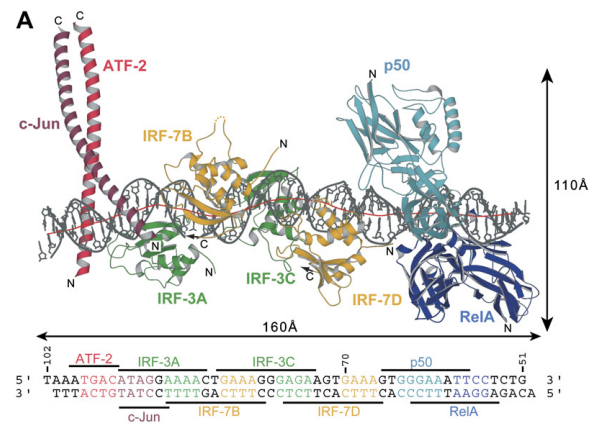
\includegraphics[width=0.8\textwidth]{enhance.png}
\end{center}

\end{frame}

\begin{frame}{The Interferon-$\beta$ Enhanceosome}

Enhanceosomes are protein complexes which solely regulate gene transcription

\end{frame}

\begin{frame}{Training on BBBC039 U2OS Cells}
\vspace{0.1in}
BBBC039: 200 images, 160 train + 40 validation, 256\;x\;256 random crop

\begin{center}
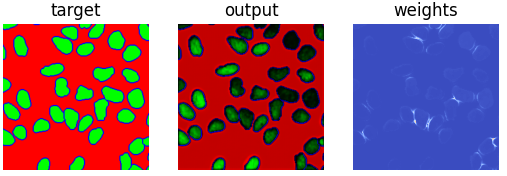
\includegraphics[width=0.8\textwidth]{weights.png}
\end{center}

We train a 3-channel semantic segmentation model with \textbf{weighted} cross-entropy loss:

\begin{equation*}
\mathcal{L} = \sum_{i,j} w_{ij}\log p_{ij}(\tilde{x}) = \sum_{i,j} w_{ij}\log \frac{\exp(-s_{ij}(\tilde{x}))}{\sum_{x\in\chi} \exp(-s_{ij}(\tilde{x}))}
\end{equation*}

$p_{ij}$ is the probability the model assigns a pixel to the true class $\tilde{x} \in \{\textrm{a}, \textrm{b}, \textrm{c}\}$

\end{frame}

\begin{frame}{Training on BBBC039 U2OS Cells}

\begin{center}
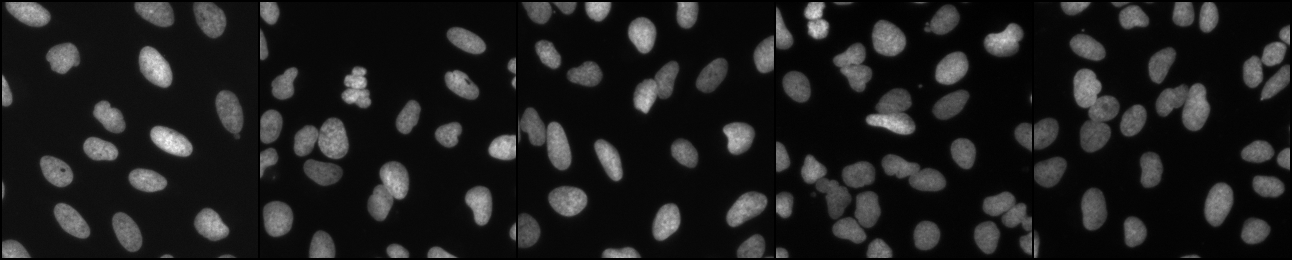
\includegraphics[width=0.85\textwidth]{input-train.png}
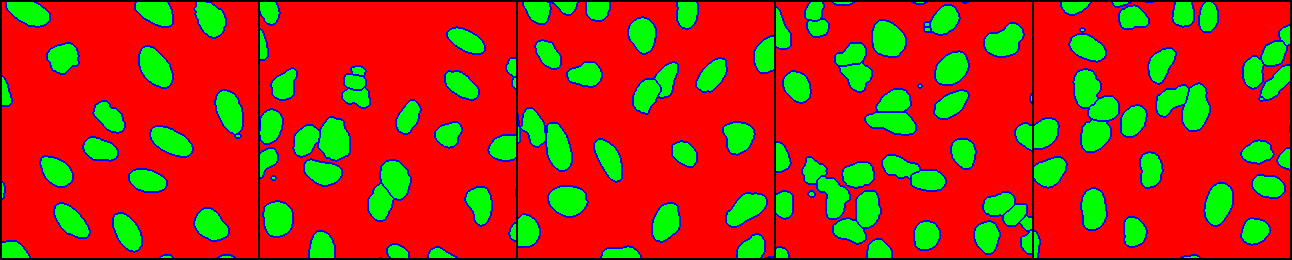
\includegraphics[width=0.85\textwidth]{target-train.png}
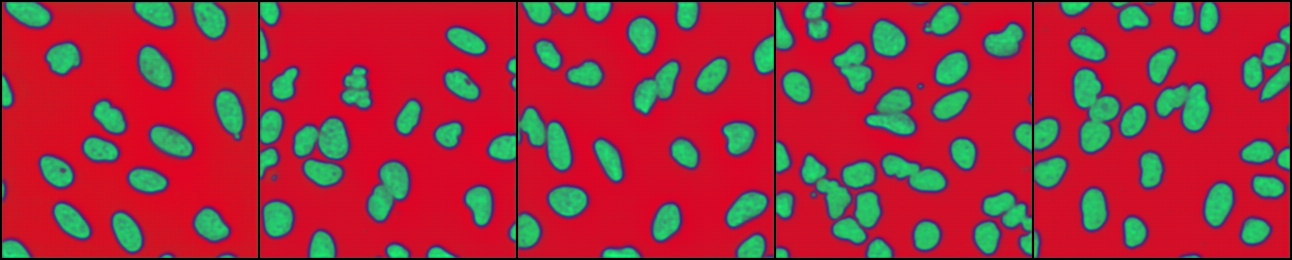
\includegraphics[width=0.85\textwidth]{output-train.png}
\end{center}

\end{frame}

\begin{frame}{Training on BBBC039 U2OS Cells}
Learning rate $\eta=0.01$, Batch-size $B=5$ (32 train iterations, 8 validation)
\begin{center}
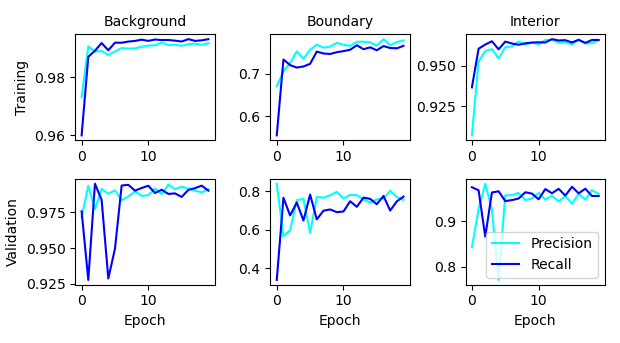
\includegraphics[width=0.85\textwidth]{metrics.png}
\end{center}

\end{frame}



% Adding the option 'allowframebreaks' allows the contents of the slide to be expanded in more than one slide.
\begin{frame}[allowframebreaks]{References}
	\tiny\bibliography{references}
	\bibliographystyle{apalike}
\end{frame}

\end{document}
